\documentclass[preprint,12pt]{elsarticle}
\usepackage{amsmath,amssymb}
\usepackage{graphicx}
\usepackage{longtable,booktabs,array,calc}
\usepackage{lineno}
\usepackage[colorlinks=true,linkcolor=blue,citecolor=blue,urlcolor=blue]{hyperref}
\providecommand{\tightlist}{\setlength{\itemsep}{0pt}\setlength{\parskip}{0pt}}
\graphicspath{{../../results/analysis/hq/}{../../results/E3_stability/hq/}}
\journal{Chaos, Solitons \& Fractals}
\begin{document}
\begin{frontmatter}
\title{Boundary symmetry as a design principle for vortex topology in thermal nonlocal media}
\author{[authors and affiliations to be added]}
\begin{abstract}
In a thermal nonlocal medium the refractive-index change is set by heat conduction, so the shape and the temperature of the sample boundary enter the nonlinear response felt by every beam inside it. We show that this makes the boundary a design tool for the topology of vortex solitons in an otherwise homogeneous material. The lowest-order anisotropy induced by a regular \(n\)-gon is given exactly by \(\delta N = U (r/\rho)^n \cos n\theta / [\pi n (n+1)]\), where \(U\) is the beam power and \(\rho\) the conformal radius of the cross-section, and polygons with equal \(\rho\) are equivalent to a disk up to this term. The discrete rotational symmetry transferred in this way transmutes a vortex of charge \(m\) according to a selection rule: the central charge, the number of satellite vortices and their radii \(r_s \propto \varepsilon^s\) follow from a Newton polygon of the angular harmonics, with fractional exponents \(s = 1, 1/2, 1/3, 1/4\) that the numerics reproduce to within 0.6\%. The boundary also controls stability. It widens the intrinsic low-power instability window of the doubly charged vortex by up to a factor of six, and the window edges are predicted quantitatively by Hamilton--Hopf collisions of disk Bogoliubov channels obeying the selection rule \(\kappa = L \bmod n\). Finally, quadrupolar boundary heating of amplitude \(\Theta\) splits the doubly charged vortex into a twin vortex with separation \(\propto \Theta^{1/2}\). The twin vortex is stable below a symmetry-breaking pitchfork at \(\Theta_c = 1.176\) and can be dragged by a rotating heating pattern. A forced-splitting-mode picture predicts, without free parameters, the free co-rotation rate after the heating is switched off, the separation response \(\omega_\mathrm{rot}/(\omega_\mathrm{rot} - 2\Omega)\) to a pattern rotating at \(\Omega\), and the locking boundaries. Co-rotation is limited by a fold before a second-order resonance; counter-rotation is limited where the symmetry-breaking translation mode reaches zero frequency in the rotating frame, \(|\Omega_c^-| \simeq \omega_\mathrm{odd} \propto (\Theta_c - \Theta)^{1/2}\).
\end{abstract}
\begin{highlights}
\item Sample boundaries transfer \(C_n\) symmetry to beams through an exact thermal law
\item A Newton-polygon rule predicts vortex transmutation and fractional scaling laws
\item Boundary symmetry widens vortex instability windows via channel collisions
\item Quadrupolar boundary heating gives a tunable, rotatable twin vortex
\item Both locking limits of the dragged twin vortex follow from identified modes
\end{highlights}
\begin{keyword}
Thermal nonlocal media \sep Vortex solitons \sep Topological charge transmutation \sep Discrete rotational symmetry \sep Krein collision \sep Hamilton–Hopf bifurcation
\end{keyword}
\end{frontmatter}
\linenumbers
\hypertarget{introduction}{%
\section{Introduction}\label{introduction}}

Optical vortex solitons, self-trapped beams that carry a phase singularity of integer charge \(m\), are a natural testbed for the interplay between topology and nonlinearity \citep{Desyatnikov2005review}. In local self-focusing media they are destroyed by azimuthal modulational instability. Nonlocal nonlinearities, in which the refractive index at a point depends on the intensity in a finite neighbourhood, can suppress this instability \citep{Malomed2022review, Rotschild2005, Kartashov2007cyl, Zhang2019higher, Shou2021cylvector}. Thermal media such as lead glass are an extreme example: the index change obeys a Poisson equation for the temperature, the range of the nonlocality is set by the sample itself, and the boundary conditions of heat conduction act on the beam over macroscopic distances \citep{Alfassi2007boundary, Alfassi2007surface, Shou2009cylforce}. Sample boundaries have accordingly been used to steer solitons \citep{Ye2009steering, Jiang2010rect, Louis2013nonsym}, to support surface solitons and vortices \citep{Ye2008surface, Kartashov2007surface}, to stabilize dipoles and multipoles \citep{Ye2008dipole, Dong2010multipole} and to shape soliton propagation in finite samples \citep{Liang2008finite, Buccoliero2009boundary}. Recent work has made solitons precess in a heptagonal sample \citep{Chen2025heptagon}, built spiralling soliton arrays from the boundary force \citep{Chen2025spiraling}, and switched vortex beams between breathing and chaotic regimes by changing the transverse size of the sample \citep{Wang2025boundarychaoticon, Li2023adaptive, Wang2022chaoticon}; engineering the thermal conductivity offers a further handle \citep{Kartashov2013thermal}. In rectangular samples a doubly charged vortex splits into a pair of unit vortices, the ``twin vortex'' \citep{Ye2010twin}.

Discrete rotational symmetry changes the topology of vortices in a well-understood way. In a medium invariant under rotations by \(2\pi/n\), angular momentum is replaced by an angular pseudomomentum \(\mu = m \bmod n\), and a vortex of charge \(m\) may ``transmute'' into a structure with a different central charge \citep{Ferrando2005vortex, GarciaMarch2009symmetry, GarciaMarch2009physd, Zacares2009}. Transmutation has been studied in photonic lattices and waveguide arrays \citep{Kartashov2023arrays, Dong2022twisted}, with symmetry-breaking optical elements in free space \citep{Novoa2014offaxis, Zhang2019metasurface} and as a means of vorticity control in condensates \citep{PerezGarcia2007}. Anisotropy also splits multiply charged vortices. In photorefractive crystals a vortex of charge \(n\) decays into \(n\) unit vortices arranged along a line fixed by the crystal anisotropy \citep{Mamaev1996pair, Mamaev1997decay}. A doubly quantized vortex in a condensate splits through a dynamical instability, a collision between positive- and negative-energy collective modes \citep{Skryabin2001, Mottonen2003split, Shin2004dqv, Kawaguchi2004split, Lundh2006, Nilsen2008splitting, Kapitula2013krein, Takeuchi2018}, whose time scale can be set by the trap anisotropy \citep{Xiong2020ring}. In all these settings the symmetry or the anisotropy is imposed by a structured medium, an optical element or a trap, and the splitting is characterized by thresholds and time scales rather than by a scaling law for the positions of the vortices.

Here the medium is homogeneous, and the discrete symmetry enters only through the boundary of the sample, via the long-range thermal response. Boundary effects in thermal media have so far been treated through the geometry of particular samples; there is no general law for how a boundary symmetry reaches the beam, and no rule for what it does to the topology of a vortex. We ask whether the boundary can serve as a systematic design principle for vortex topology, and whether a patterned boundary temperature can make that design reconfigurable. We answer both questions in five steps:

\begin{enumerate}
\def\labelenumi{\arabic{enumi}.}
\tightlist
\item
  \textbf{Symmetry transfer} (Sec. 3). The boundary symmetry reaches the beam through an exact law. The leading anisotropy depends only on the beam power and the conformal radius of the cross-section, and samples with equal conformal radius are equivalent.
\item
  \textbf{Selection rule and scaling} (Sec. 4). The transferred symmetry transmutes the vortex according to a selection rule. A Newton-polygon construction gives the central charge, the satellite rings and fractional scaling laws for their radii, all confirmed numerically.
\item
  \textbf{Stability} (Sec. 5). The boundary shapes the stability of the transmuted states. The low-power instability window of the \(m = 2\) vortex is widened by boundary symmetry, and the window edges follow from Hamilton--Hopf collisions of disk Bogoliubov channels obeying a selection rule.
\item
  \textbf{Observability} (Sec. 6). Transmutation is fast compared with the growth of the instabilities, which defines an observable window.
\item
  \textbf{Thermal reconfiguration} (Sec. 7). Quadrupolar boundary heating produces a tunable twin vortex. Its statics, its pitchfork instability and its response to a rotating heating pattern are described quantitatively by one forced-oscillator picture.
\end{enumerate}

To our knowledge, the transfer law and the conformal-radius universality, the fractional scaling of the satellite positions, the boundary-induced widening of instability windows with its channel selection rule, and the use of patterned boundary heating to reconfigure and drag vortex structures have no precedent. The group-theoretical skeleton of the selection rule is the one known for lattices \citep{Ferrando2005vortex, Zacares2009}, and the twin vortex itself is the structure found in rectangular samples \citep{Ye2010twin}. What is new is that both follow here from the boundary alone, with quantitative laws, and can be tuned continuously and switched in situ.

\hypertarget{model}{%
\section{Model}\label{model}}

We consider a continuous-wave beam with dimensionless amplitude \(q(x, y, \xi)\) propagating along \(\xi\) in a thermal medium of cross-section \(\mathcal{D}\), in the standard normalization of Refs. \citep{Ye2010twin, Ye2008surface}:
\[
i\,\partial_\xi q = -\tfrac12 \nabla_\perp^2 q - N q, \qquad
\nabla_\perp^2 N = -|q|^2 \quad \text{in } \mathcal{D}, \qquad N = N_b \ \text{on } \partial\mathcal{D} .
\tag{1}
\]
Here \(N\) is the thermally induced refractive-index change. The sample boundary is held at a prescribed temperature, so \(N_b = 0\) for a uniform heat sink and \(N_b = \Theta \cos n(\theta - \theta_0)\) for a patterned boundary temperature (Sec. 7). The field vanishes outside the sample. Transverse coordinates are measured in units of a beam scale \(r_0\), the propagation distance in units of the diffraction length \(k r_0^2\), and the power \(U = \iint |q|^2\,dx\,dy\) is proportional to the physical power \citep{Ye2008surface}. Stationary states are \(q = w(x, y) e^{i b \xi}\) with propagation constant \(b\). Their linear stability follows from the Bogoliubov problem for perturbations \((u, v) e^{\lambda \xi}\).

The samples are regular \(n\)-gons (\(n = 3\)--6), a \(20 \times 40\) rectangle and disks. Polygons and the reference disk are compared at equal conformal radius \(\rho = 8\); heated disks have radius \(R = 10\). Equation (1) is invariant under \(q(x, y, \xi) \to s^2 q(sx, sy, s^2\xi)\), which maps a sample of size \(\rho\) onto one of size \(\rho/s\) with \(b \to s^2 b\), \(U \to s^2 U\) and \(\Theta \to s^2 \Theta\). All thresholds therefore depend on \(b\rho^2\) only. Numerical methods are summarized in Appendix A. All results quoted below were obtained on a grid of spacing \(h = 0.1\) (\(h = 0.15\) for the rectangle); key results were checked on coarser and finer grids (Appendix B). Structural statements are made only when a satellite ring is larger than \(2h\) (Appendix B).

\hypertarget{symmetry-transfer-from-the-boundary-to-the-beam}{%
\section{Symmetry transfer from the boundary to the beam}\label{symmetry-transfer-from-the-boundary-to-the-beam}}

Let \(f\) map \(\mathcal{D}\) conformally onto the unit disk with \(f(0) = 0\) and \(f'(0) = 1/\rho\), which defines the conformal radius \(\rho\). The Dirichlet Green function of Eq. (1) is \(G(z, z') = (2\pi)^{-1} \ln |(1 - f(z)\overline{f(z')}) / (f(z) - f(z'))|\). For a regular \(n\)-gon the Schwarz--Christoffel map gives \(f(z) = (z/\rho)[1 + c_n (z/\rho)^n + \dots]\) with \(c_n = -2/[n(n+1)]\). Expanding \(G\) for \(|z|, |z'| \ll \rho\) and integrating against a beam whose intensity has \(C_n\) symmetry gives
\[
N(z) = N_\mathrm{free}(z) + \frac{U}{2\pi} \ln \rho + \frac{U}{\pi n (n+1)} \left( \frac{r}{\rho} \right)^{n} \cos n\theta + \dots ,
\tag{2}
\]
where \(N_\mathrm{free}\) is the response of an unbounded medium. Equation (2) contains two statements:

\begin{itemize}
\tightlist
\item
  \textbf{Transfer law.} The lowest anisotropic term depends only on the total power and on \(\rho\), not on the beam shape. Only angular harmonics \(0, n, 2n, \dots\) appear.
\item
  \textbf{Conformal-radius universality.} The isotropic part differs from that of free space only by the constant \((U/2\pi) \ln \rho\), which shifts \(b\). Polygons with equal \(\rho\) therefore support the same family \(U(b)\) of \(C_n\)-symmetric states up to \(O((r/\rho)^n)\).
\end{itemize}

Figure 1 confirms both statements. The numerically extracted \(n\)-th harmonic of \(N\), normalized by \(U/[\pi n (n+1)]\), collapses onto \((r/\rho)^n\) for \(n = 3\)--6 and \(\rho = 6\)--18 without fitting. The ratio to theory lies within \(0.99997\)--\(1.004\), independent of beam shape and power to \(1.6 \times 10^{-5}\). The power curves \(U(b)\) of the four polygons and the disk at \(\rho = 8\) coincide to \(3.7 \times 10^{-4}\) for \(m = 0\). The boundary therefore acts on a centred beam as a weak, analytically known \(C_n\) perturbation of strength
\[
\varepsilon_\mathrm{shape} = \frac{U}{\pi n (n+1) \rho^n}, \qquad
\varepsilon_\mathrm{heat} = \frac{\Theta}{R^n},
\tag{3}
\]
where the second expression is the harmonic field \(\Theta (r/R)^n \cos n(\theta - \theta_0)\) produced in a disk by the boundary temperature \(\Theta \cos n(\theta - \theta_0)\). Unlike the shape anisotropy, the heating anisotropy is independent of the beam power, can have either sign and can be rotated.

\begin{figure}[tbp]
\centering
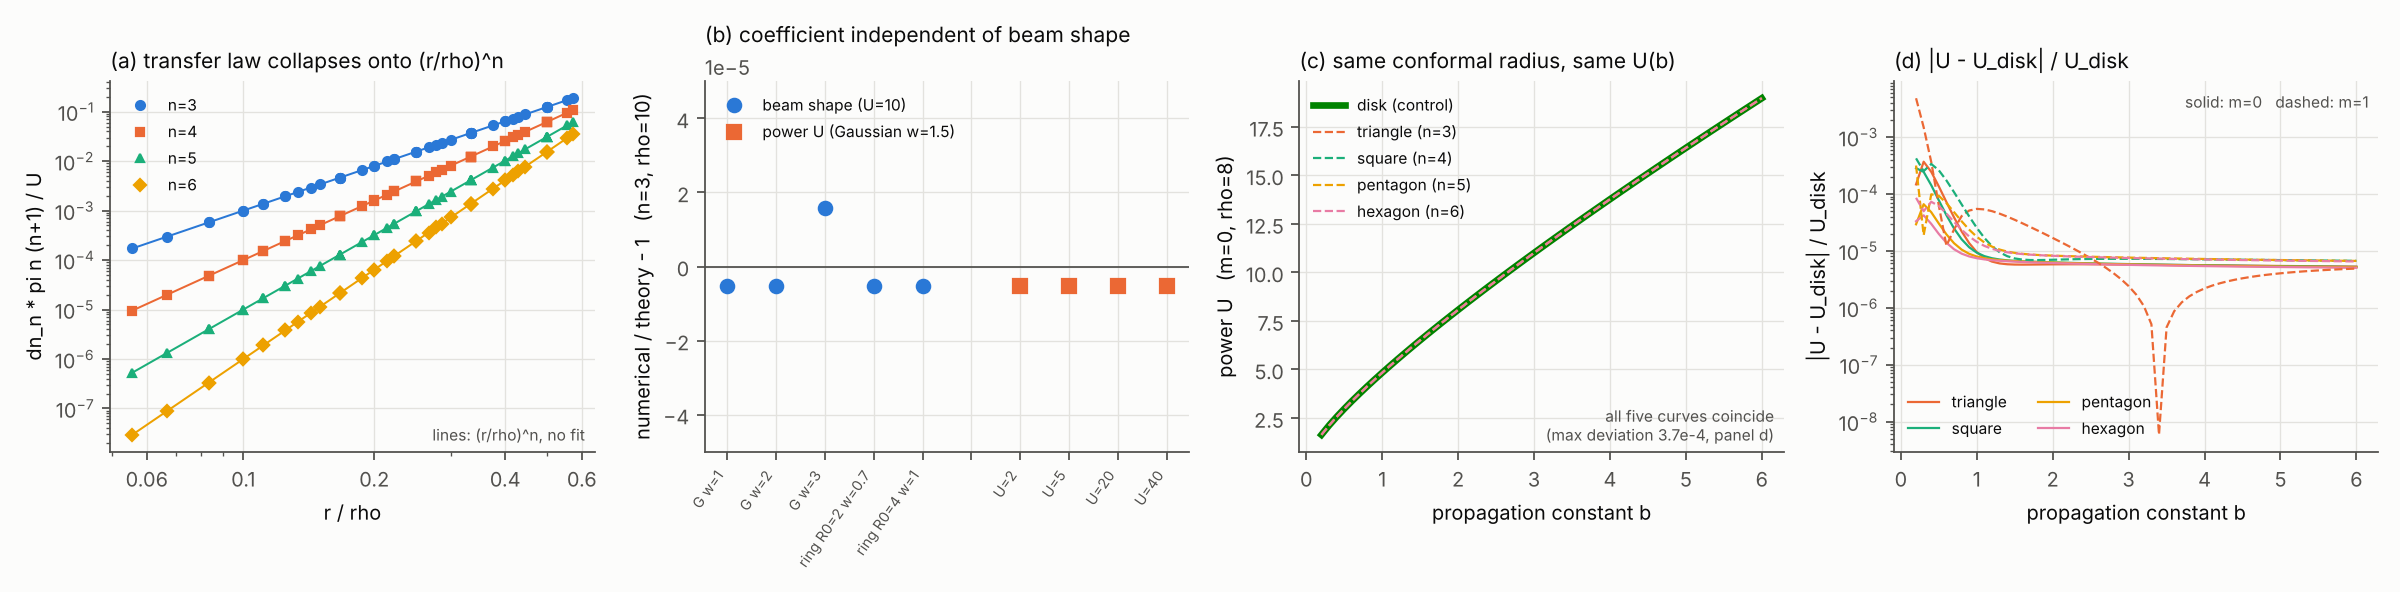
\includegraphics[width=0.98\textwidth,height=0.72\textheight,keepaspectratio]{symmetry_transfer.png}
\caption{\textbf{Symmetry transfer.}
(a) The \(n\)-th angular harmonic of the thermal index, \(\delta N_n \cdot \pi n (n+1)/U\), versus \(r/\rho\) for \(n = 3\)--6 and \(\rho = 6\)--18. Lines are \((r/\rho)^n\) (no fit).
(b) Ratio of numerical to theoretical coefficient for Gaussian and ring beams of different widths and for powers \(U = 2\)--40.
(c) Power curves \(U(b)\) of \(m = 0\) states in four regular polygons and the disk at equal conformal radius \(\rho = 8\).
(d) Relative deviation from the disk curve for \(m = 0\) (solid) and \(m = 1\) (dashed).}
\label{fig1}
\end{figure}


\hypertarget{transmutation-selection-rule-and-fractional-scaling}{%
\section{Transmutation selection rule and fractional scaling}\label{transmutation-selection-rule-and-fractional-scaling}}

\textbf{Angular pseudomomentum.} If the sample and its boundary temperature are invariant under rotation by \(2\pi/n\), the charge-\(m\) vortex belongs to the irreducible representation \(\mu = m \bmod n\). Its field contains only the angular harmonics \(l_j = m - j n\) (and \(m + j n\)), \(w = \sum_j w_{l_j}(r) e^{i l_j \theta}\), with regular behaviour \(w_l \simeq a_l r^{|l|}\) at the centre. Each action of the perturbation \(\varepsilon r^n \cos n\theta\) shifts the angular momentum by \(\pm n\), so \(a_{l_j} = O(\varepsilon^j)\).

\textbf{Newton polygon.} At radius \(r\) the harmonic with the largest \(|a_{l_j}| r^{|l_j|} \sim \varepsilon^j r^{|l_j|}\) dominates the phase. As \(r \to 0\), the dominant harmonic moves along the lower convex hull of the points \(\{(|l_j|, j)\}\), from \((|m|, 0)\) to the point of smallest \(|l|\). This gives the following rules:

\begin{itemize}
\tightlist
\item
  The \textbf{central charge} \(v\) is the \(l\) at the end of the hull, i.e.~the harmonic with the smallest \(|l|\) (smallest \(j\) in case of a tie).
\item
  Each hull edge \((|l_a|, j_a) \to (|l_b|, j_b)\) is a \textbf{ring of satellite vortices} of total charge \(l_a - l_b\), arranged with \(C_n\) symmetry.
\item
  Each ring has radius \(r_s \propto \varepsilon^{s}\) with \(s = (j_b - j_a)/(|l_a| - |l_b|)\).
\end{itemize}

Some examples:

\begin{longtable}[]{@{}llll@{}}
\toprule\noalign{}
\((n, m)\) & central charge & satellites & \(r_s\) scaling \\
\midrule\noalign{}
\endhead
\bottomrule\noalign{}
\endlastfoot
(2, 2) & \(0\) & \(2 \times (+1)\) & \(\varepsilon^{1/2}\) (twin vortex) \\
(3, 2) & \(-1\) & \(3 \times (+1)\) & \(\varepsilon^{1}\) \\
(3, 3) & \(0\) & \(3 \times (+1)\) & \(\varepsilon^{1/3}\) \\
(4, 3) & \(-1\) & \(4 \times (+1)\) & \(\varepsilon^{1/2}\) \\
(4, 4) & \(0\) & \(4 \times (+1)\) & \(\varepsilon^{1/4}\) \\
\end{longtable}

The exponent \(s = 1/(|m| - |v|)\) can be small, so high-charge vortices are hypersensitive to weak anisotropy.

\textbf{Atlas.} Figure 2 shows the stationary states at \(b \approx 1\) for six samples and \(m = 1\)--6. Of the 36 families, 31 agree with the rule in central charge and satellite number. In two the satellite ring is below the resolution limit: the triangle with \(m = 2\) (\(r_s = 0.198 \approx 2h\) at \(b = 1\)) and the pentagon with \(m = 3\) (\(r_s = 0.06\)). The remaining three are the disk controls with \(m = 4\)--6. They read central charges \(0, 1, 2 = m - 4\) with satellite rings at \(r \approx 0.3\), the transmutation induced by the \(C_4\) symmetry of the square grid itself. This sets a floor below which no structural claim is made for \(m \ge 4\) (Appendix B); for the same reason the rules for \(n = 5, 6\) are demonstrated with boundary heating, whose anisotropy can be made much larger than the grid error.

\textbf{Fractional scaling.} Combining the rule with Eq. (3), at fixed power \(r_s \propto \rho^{-ns}\) for shaped samples and \(r_s \propto \Theta^{s}\) for heated disks. Figure 3 shows the local exponents in the asymptotic regime \(r_s / r_\mathrm{ring} \to 0\). For shaped samples they are \(-3.001\), \(-1.000\), \(-1.988\) and \(-0.999\) for \((n, m) = (3, 2)\), \((3, 3)\), \((4, 3)\) and \((4, 4)\), against the predicted \(-3, -1, -2, -1\). For heated disks they are \(0.500, 1.000, 0.333, 0.499, 1.000, 0.500\) for \((2, 2), (3, 2), (3, 3), (4, 3), (5, 3), (6, 4)\). Reversing the sign of \(\Theta\) rotates the satellite ring by \(\pi/n\). Global power-law fits that include large rings deviate (for example \(-0.74\) instead of \(-1\) for (4, 4)), because those points leave the perturbative regime; the asymptotic exponents are unaffected.

\begin{figure}[tbp]
\centering
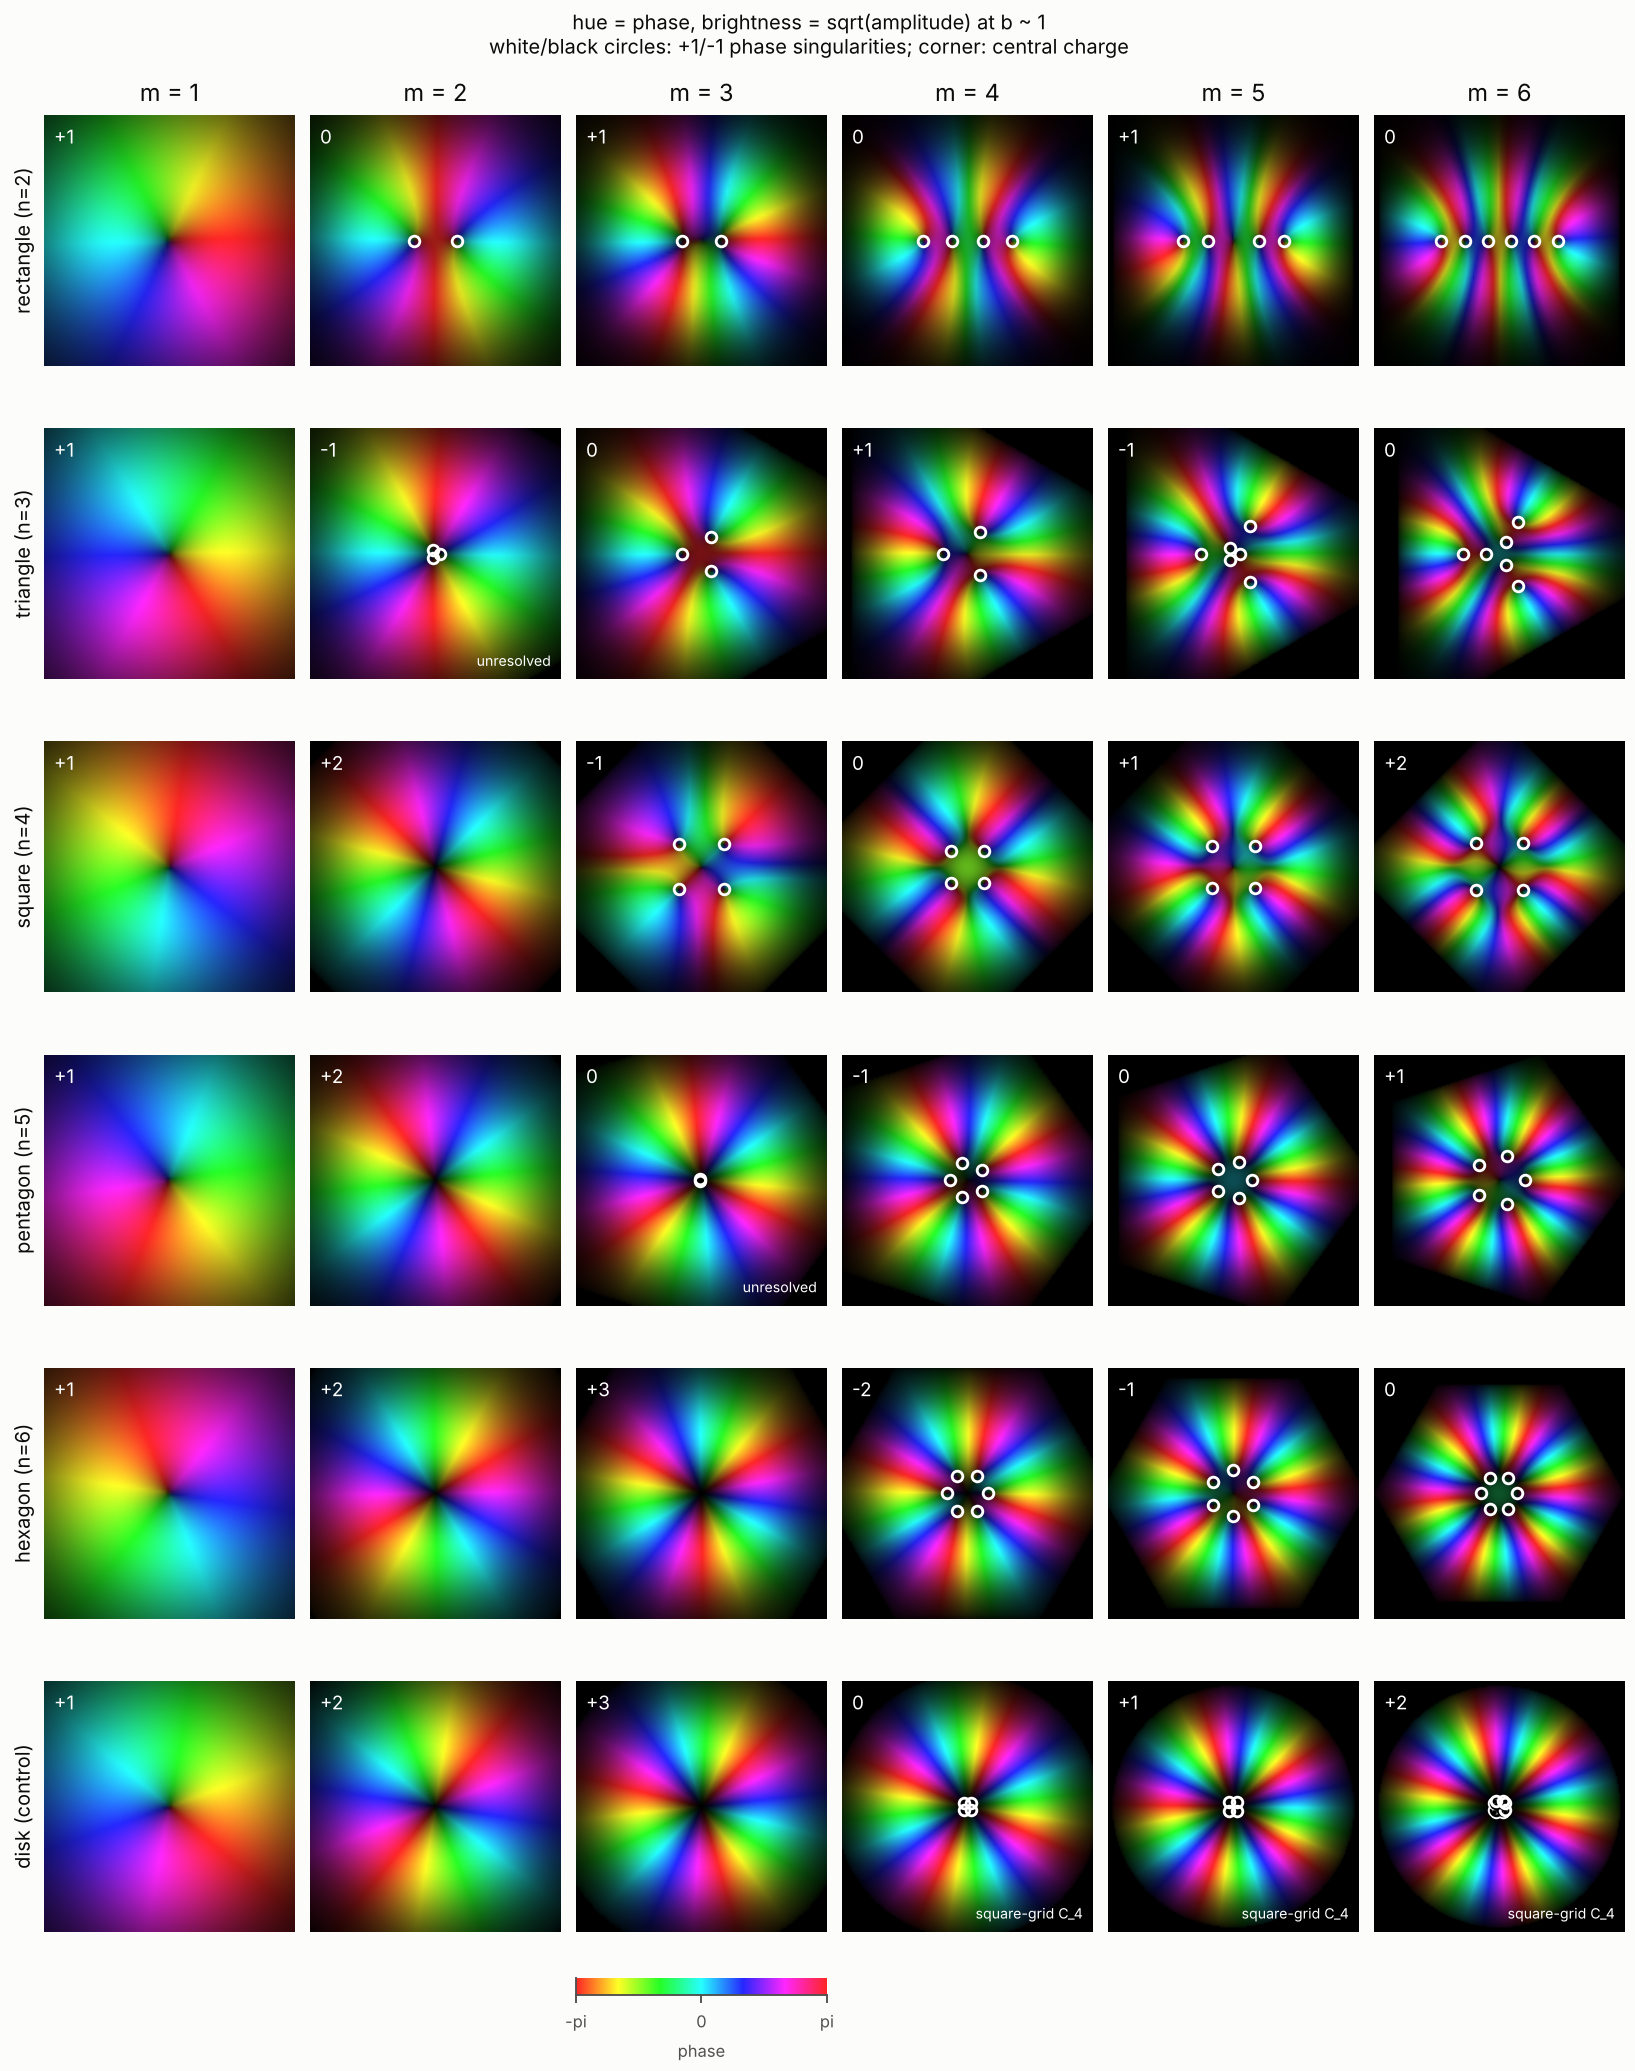
\includegraphics[width=0.98\textwidth,height=0.72\textheight,keepaspectratio]{atlas_fields.png}
\caption{\textbf{Transmutation atlas.} Stationary vortex states with \(m = 1\)--6 (columns) in a \(20\times40\) rectangle, regular \(n\)-gons with \(\rho = 8\) and the disk (rows), at \(b \approx 1\). Hue is the phase and brightness is the square root of the amplitude; white and black circles mark \(+1\) and \(-1\) singularities; the number in the corner is the central charge. ``Unresolved'' marks satellite rings smaller than \(2h\). The disk cells with \(m \ge 4\) show the splitting induced by the square grid's own \(C_4\) symmetry, used as a control.}
\label{fig2}
\end{figure}


\begin{figure}[tbp]
\centering
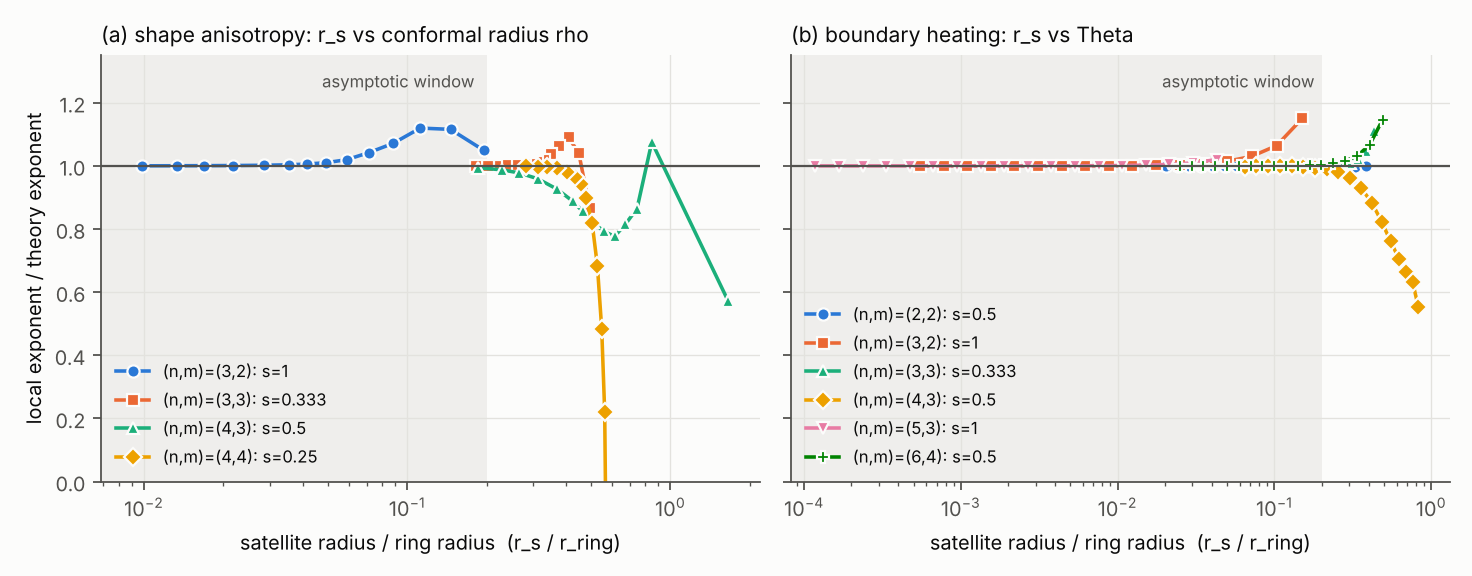
\includegraphics[width=0.98\textwidth,height=0.72\textheight,keepaspectratio]{scaling_local_slopes.png}
\caption{\textbf{Fractional scaling laws.} Local exponents of the satellite radius, normalized by the Newton-polygon prediction, versus \(r_s / r_\mathrm{ring}\).
(a) Shaped samples, \(r_s \propto \rho^{-ns}\).
(b) Boundary heating, \(r_s \propto \Theta^{s}\), for \((n, m) = (2,2), (3,2), (3,3), (4,3), (5,3), (6,4)\).
The shaded region is the asymptotic window.}
\label{fig3}
\end{figure}


\hypertarget{stability-boundary-widened-windows-and-their-mechanism}{%
\section{Stability: boundary-widened windows and their mechanism}\label{stability-boundary-widened-windows-and-their-mechanism}}

\textbf{Overview}. Figure 4(c) shows the stability of the \(m = 2\) families. Every sample shares the intrinsic window of the disk: the \(m = 2\) vortex is unstable at low power through the \(L = -2\) splitting mode (\(u \propto e^{0 i \theta}\), \(v \propto e^{-4 i \theta}\)). An independent radial solver for the disk, which uses no Cartesian grid (Appendix B, Fig. S1), places the edge at \(bR^2 = 32.56\), converged in the radial resolution; the Cartesian grids give \(31.8\) (\(h = 0.1\)) and \(32.2\) (\(h = 0.05\)). The instability is dynamically real: a noise-seeded \(m = 2\) state at \(b\rho^2 = 12.8\) breaks up within \(\xi = 1000\) on two grids, whereas states at \(b\rho^2 = 38\)--51 survive. Ref. \citep{Kartashov2007cyl} states that vortices with \(m \le 2\) in cylindrical thermal media are stable in their whole existence domain, for any \(b\). That work uses the same model, normalization and boundary condition, but shows no stability data for \(m = 2\) and specifies no scan range. Our results agree with the statement above the window, \(bR^2 > 32.6\), and add a narrow low-power window (\(b < 0.020\) for the radius \(R = 40\) used there) that is not covered by the data shown in Ref. \citep{Kartashov2007cyl}.
The boundary widens this window in a shape-specific way:

\begin{longtable}[]{@{}
  >{\raggedright\arraybackslash}p{(\columnwidth - 2\tabcolsep) * \real{0.5000}}
  >{\raggedright\arraybackslash}p{(\columnwidth - 2\tabcolsep) * \real{0.5000}}@{}}
\toprule\noalign{}
\begin{minipage}[b]{\linewidth}\raggedright
sample
\end{minipage} & \begin{minipage}[b]{\linewidth}\raggedright
upper edge of the \(m = 2\) window (at \(\rho = 8\))
\end{minipage} \\
\midrule\noalign{}
\endhead
\bottomrule\noalign{}
\endlastfoot
disk, pentagon & \(0.494\)--\(0.500\) (the intrinsic window) \\
hexagon & \(0.744\)--\(0.750\) \\
square & \(0.925\)--\(0.931\) \\
triangle & \(2.72\) at \(h = 0.1\); \(2.95\)--\(2.99\) in the continuum limit \\
\(20\times40\) rectangle (\(\rho = 12.64\)) & \(b_c \rho^2 = 79.4\), i.e.~\(1.24\) at \(\rho = 8\), \(2.5\times\) the disk value \\
\end{longtable}

For \(m = 1\), the disk is unstable only at very low power (\(bR^2 < 8.25\) from the radial solver, \(L = -1\); \(b < 0.13\) at \(\rho = 8\)), the triangle up to \(b = 0.73\) (\(|\kappa| = 1\)), and all other samples are stable for \(b \ge 0.2\). For \(m \ge 3\), all samples are unstable at all \(b\). The growth rates at high power are independent of the sample (0.229, 0.294, 0.334, 0.40 for \(m = 3\)--6 at \(b = 7\)), so boundary symmetry does not stabilize higher-order transmuted states.

\textbf{Mechanism: channel collisions with a selection rule}. In the disk, Bogoliubov modes with different angular index \(L\) (\(u \propto e^{i(m+L)\theta}\), \(v \propto e^{i(L-m)\theta}\)) do not couple. Each branch carries a Krein signature, the sign of \(\|u\|^2 - \|v\|^2\). A \(C_n\) boundary couples \(L\) only to \(L + kn\), so the index \(\kappa = L \bmod n\) is conserved. An instability window opens, or widens, wherever a Krein-positive branch \(L\) and a Krein-negative branch \(L + kn\) of the disk spectrum cross or come close (Hamilton--Hopf). This explains all four cases quantitatively {[}Fig. 4(a){]}:

\begin{itemize}
\tightlist
\item
  \textbf{Hexagon.} The unstable mode in the extended part of the window (0.55--0.74) contains 36--40\% of \(L = +4\), and the disk branches \(L = -2\) (K\(+\)) and \(L = +4\) (K\(-\)) cross exactly there.
\item
  \textbf{Pentagon.} The partner \(L = +3\) never approaches \(L = -2\) (mixing \(\le 1.6\%\)), so the window equals that of the disk.
\item
  \textbf{Square.} The partners \(L = +2\) and \(L = +6\) cross \(L = -2\) near \(b \approx 0.55\)--0.65. They dominate in turn, which makes the growth rate non-monotonic.
\item
  \textbf{Edge criterion.} The two-mode Hamilton--Hopf criterion \(|\Delta\omega_\mathrm{disk}(b)| = 2 g\) predicts the edges at 0.78 (hexagon) and between 0.85 and 0.95 (square), against the measured 0.744 and 0.925.
\end{itemize}

The exceptionally wide triangle window {[}Fig. 4(b){]} is a \(\kappa = 0\) pair, \(L = -3\) (K\(+\)) and \(L = 0\) (K\(-\)). The two branches cross near \(b \approx 0.7\) and remain nearly degenerate (\(\Delta\omega = 0.019\)--0.038 up to \(b = 3.4\)), so the weak \(C_3\) coupling locks them into instability over a wide range of \(b\). Three observations confirm this picture:

\begin{itemize}
\tightlist
\item
  The unstable-mode frequency equals the mean of the two disk branches to within 0.14\% on four grids.
\item
  The coupling extracted from the growth rate, \(g = [\gamma^2 + (\Delta\omega/2)^2]^{1/2}\), is constant to 7\% across the window.
\item
  The criterion \(\Delta\omega(b_c) = 2g\) predicts \(b_c = 2.93\), against the extrapolated edge 2.95--2.99.
\end{itemize}

The grid dependence of the triangle edge (2.46, 2.72, 2.81, 2.91 for \(h = 0.15\), 0.1, 0.075, 0.05) comes entirely from the \(h^2\) convergence of \(g\), because \(\Delta\omega\) varies slowly with \(b\).

\textbf{Heated disks: a tunable coupling}. Boundary heating replaces the fixed shape anisotropy by a tunable one and tests the mechanism directly:

\begin{itemize}
\tightlist
\item
  \textbf{Linear law.} For \(C_3\) heating of the \(m = 1\) vortex at small \(\Theta\), the maximum growth rate is \(0.150\,\Theta\) to within 1.5\% (\(\Theta = 0.02\)--0.16), and \(\gamma/\Theta\) collapses onto a single curve {[}Fig. 4(d){]}. The window is centred at the crossing of the disk branches \(L = -2\) and \(L = +1\) and has a width proportional to \(\Theta\).
\item
  \textbf{High-\(b\) window of \(C_3\)-heated \(m = 2\).} This window comes from the same \(L = -3/L = 0\) pair as the triangle window. The coupling extracted at five \(\Theta\) collapses onto \(c(b)\,\Theta\) with \(c \propto r_\mathrm{ring}^3\) to 1\%, i.e.~\(g \simeq 2.04\,\Theta\,(r_\mathrm{ring}/R)^3\): the coupling is the heating field evaluated at the bright ring.
\item
  \textbf{Edge predictions.} The Hamilton--Hopf criterion gives the upper edges as 3.358, 4.207, 4.920, 5.545 for \(\Theta = 1\), 1.5, 2, 2.5, against the measured 3.359, 4.209, 4.922, 5.547.
\end{itemize}

\begin{figure}[tbp]
\centering
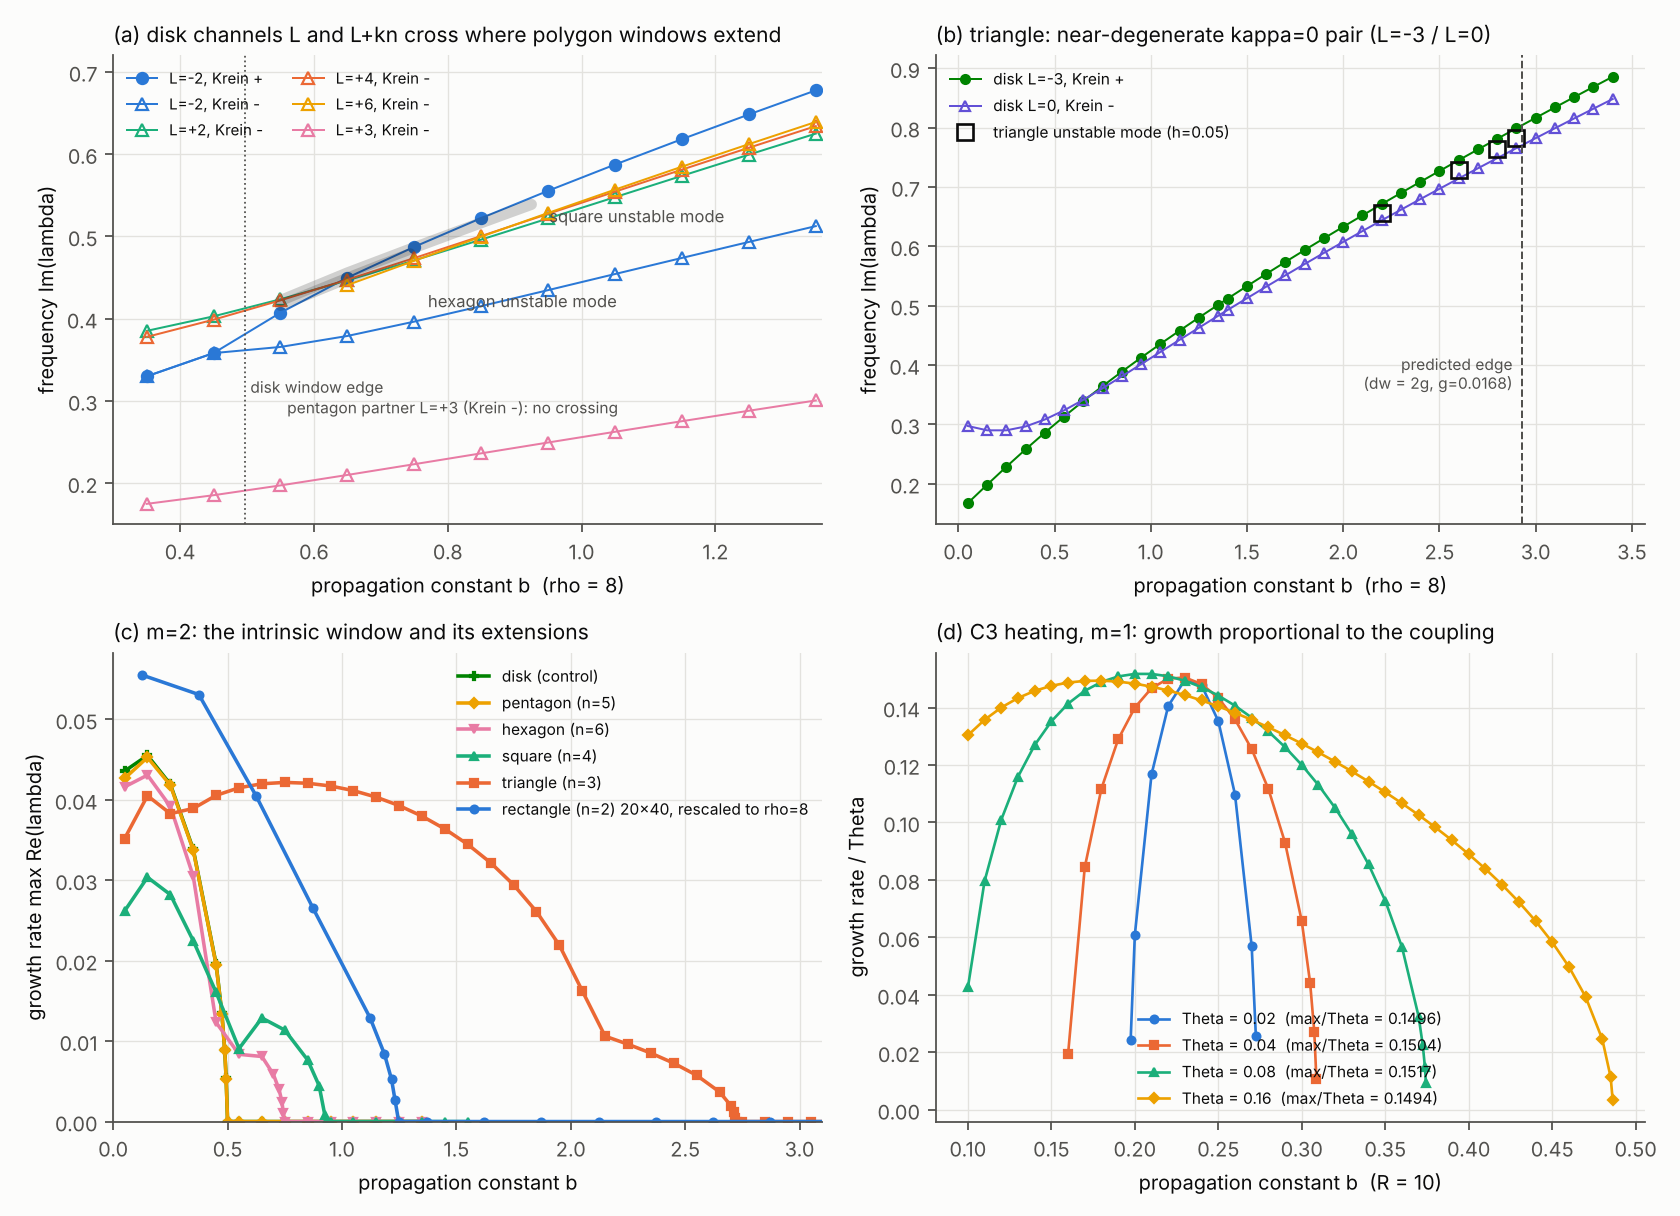
\includegraphics[width=0.98\textwidth,height=0.72\textheight,keepaspectratio]{window_mechanism.png}
\caption{\textbf{Mechanism of the instability windows.}
(a) Disk Bogoliubov channels: Krein-positive \(L = -2\) and Krein-negative partners \(L = +2, +4, +6, +3\), with the unstable-mode frequencies of the square and hexagon.
(b) Triangle: the near-degenerate \(\kappa = 0\) pair \(L = -3\)/\(L = 0\), the unstable-mode frequency (\(h = 0.05\)) and the Hamilton--Hopf edge prediction.
(c) Maximum growth rate of \(m = 2\) states in all samples; the rectangle is rescaled to \(\rho = 8\).
(d) \(C_3\)-heated disk, \(m = 1\): growth rate divided by \(\Theta\) for \(\Theta = 0.02\)--0.16.}
\label{fig4}
\end{figure}


\hypertarget{dynamics-and-observability}{%
\section{Dynamics and observability}\label{dynamics-and-observability}}

Since \(\mu\) is conserved by Eq. (1) in a \(C_n\)-symmetric sample, a Laguerre--Gaussian beam of charge \(m\) launched into the sample transmutes dynamically into the stationary structure. The core forms within \(\xi_{t} \approx 2\)--12 diffraction lengths for all samples {[}Fig. 5(a){]}.

\begin{itemize}
\tightlist
\item
  \textbf{Stable regime.} For the triangle with \(m = 2\) at \(U = 25\) and 30 (\(b = 3.94\) and 5.17, above \(b_c \approx 3.0\)), the transmuted structure persists to \(\xi = 600\) on two grids.
\item
  \textbf{Grid forcing, not instability.} The weight outside the input representation grows only algebraically, as \(\xi^{1.0-1.5}\), from \(10^{-13}\) to at most \(1.5\times10^{-5}\). This growth is forced by the \(C_4\) symmetry of the square grid: it is 15 times smaller at \(h = 0.05\), close to the \(h^2\) ratio. It is absent when the stationary state itself is launched, and it does not grow with 1\% input noise.
\item
  \textbf{Unstable regime.} Symmetry breaking is the linear instability amplifying its seed, with the weight growing as \(e^{2\gamma \xi}\) {[}Fig. 5(b){]}. For the disk with \(m = 3\), the fitted rate is 0.1047 against the linear 0.1048, with a breakup at \(\xi = 290\)/296 on two grids from round-off seeds. For the triangle at \(U = 15\) with input noise \(10^{-5}\) and \(10^{-3}\), the fitted rates are 0.027 and 0.030 against the linear 0.029.
\end{itemize}

In all unstable cases the transmutation distance is much shorter than the breakup distance \(\xi_b \approx 66\)--300 {[}Fig. 5(c){]}. The transmuted structure is therefore observable over realistic sample lengths even where the stationary state is linearly unstable.

\begin{figure}[tbp]
\centering
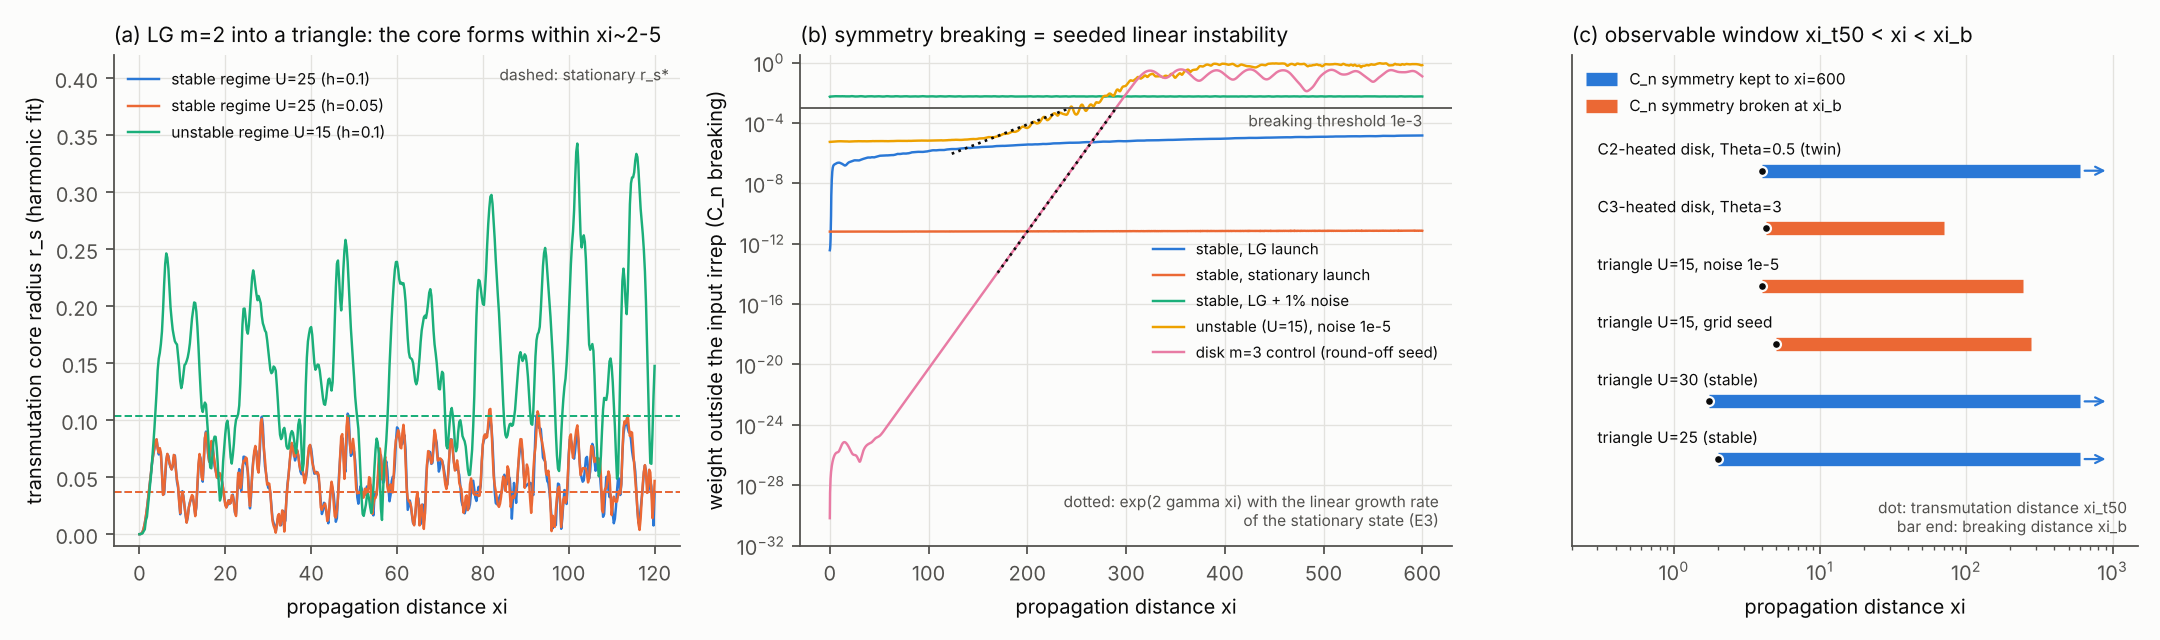
\includegraphics[width=0.98\textwidth,height=0.72\textheight,keepaspectratio]{dynamic_window.png}
\caption{\textbf{Dynamic transmutation and observability.}
(a) Core radius after launching a Laguerre--Gaussian \(m = 2\) beam into a triangle, in the stable (\(U = 25\), two grids) and unstable (\(U = 15\)) regimes; dashed lines mark the stationary values.
(b) Weight outside the input representation: algebraic growth in the stable regime and seeded exponential growth in the unstable regime. Dotted lines are \(e^{2\gamma\xi}\) with the linear growth rates.
(c) Transmutation distance (dots) and symmetry-breaking distance (bar ends) for representative cases.}
\label{fig5}
\end{figure}


\hypertarget{thermally-reconfigurable-twin-vortex}{%
\section{Thermally reconfigurable twin vortex}\label{thermally-reconfigurable-twin-vortex}}

Quadrupolar boundary heating \(N_b = \Theta \cos 2(\theta - \theta_0)\) of a disk (\(R = 10\)) at power \(U = 15\) (\(b \approx 2.29\), far above the intrinsic window) realizes the case \((n, m) = (2, 2)\) with a tunable anisotropy.

\hypertarget{splitting-tunability-and-a-symmetry-breaking-pitchfork}{%
\subsection{Splitting, tunability and a symmetry-breaking pitchfork}\label{splitting-tunability-and-a-symmetry-breaking-pitchfork}}

The doubly charged vortex splits into a central charge 0 and two unit vortices on the axis \(\theta_0 + \pi/2\), perpendicular to the hottest boundary points (Fig. 6, top row). Their half-separation follows \(r_s \propto \Theta^{1/2}\) (asymptotic exponent 0.500) and reaches \(r_s = 0.63\) and 0.83 at \(\Theta = 0.5\) and 1, i.e.~6--8 grid spacings, directly resolved {[}Fig. 6(a){]}. At \(U = 15\) the twin vortex is stable for all \(\Theta \le 1.1\) {[}Fig. 6(b){]}. The stability limit is a pitchfork bifurcation that breaks \(C_2\). The mode responsible is a rigid translation of the pair (\(\kappa = 1\), \(u \propto e^{3 i \theta}\), Krein negative), whose frequency softens with \(\omega_\mathrm{odd}^2 = 0.0238 - 0.0202\,\Theta\), exactly linear for \(\Theta = 0\)--1.1. It vanishes at \(\Theta_c = 1.176\) {[}Fig. 6(c){]}. Independent stability calculations above \(\Theta_c\) give growth rates \(0.02165\), \(0.04984\), \(0.08070\) at \(\Theta = 1.2\), 1.3, 1.5, agreeing to three digits with the extrapolation \((-\omega_\mathrm{odd}^2)^{1/2} = 0.020\), \(0.049\), \(0.080\).

\hypertarget{forced-splitting-mode-picture}{%
\subsection{Forced-splitting-mode picture}\label{forced-splitting-mode-picture}}

The disk's \(L = -2\) channel (\(u \propto e^{0 i\theta}\), \(v \propto e^{-4 i\theta}\), frequency \(\omega_{-2}\)) is precisely the mode that splits a doubly charged vortex into two unit vortices. Quadrupolar heating acting on \(f(r) e^{2 i \theta}\) generates components that project onto this channel. The twin vortex is therefore the static forced response of the splitting mode: near the centre \(w \simeq a r^2 e^{2 i \theta} + c\) with \(c \propto \Theta e^{2 i \theta_0}\), and the two zeros sit at \(r_s = (|c|/a)^{1/2} \propto \Theta^{1/2}\). Following the mode continuously in \(\Theta\) gives its frequency in the heated state, \(\omega_\mathrm{rot} = 0.2523\), 0.2558, 0.2657, 0.2808, 0.3000 for \(\Theta = 0\), 0.25, 0.5, 0.75, 1. This picture makes three parameter-free predictions:

\begin{enumerate}
\def\labelenumi{\arabic{enumi}.}
\tightlist
\item
  \textbf{Free co-rotation.} When the heating is switched off, \(c(\xi) = c_0 e^{i \omega_{-2} \xi}\), and the pair axis rotates at \(\omega_{-2}/2 = 0.1262\). The measured rate is 0.1278 at \(\Theta = 0.5\), a deviation of 1.3\% {[}Fig. 6(f){]}.
\item
  \textbf{Separation response.} A pattern rotating as \(\theta_0 = \Omega\xi\) drives the mode at frequency \(2\Omega\). The forced amplitude, and hence the squared separation, is amplified by
  \[ \frac{\langle r_s^2 \rangle}{r_{s0}^2} = \frac{\omega_\mathrm{rot}}{\omega_\mathrm{rot} - 2\Omega}. \tag{4} \]
  For locked states with \(|\Omega| \le 0.1\) away from the second-order resonance, the measured ratio agrees with Eq. (4) to within 4.2\% (\(\Theta = 0.25\)) and 4.0\% (\(\Theta = 0.5\)) {[}Fig. 6(e){]}.
\item
  \textbf{Chirality.} Co-rotation with the pair's own free rotation (\(\Omega > 0\)) meets resonances: first order at \(\Omega_1 = \omega_\mathrm{rot}/2 \approx 0.13\)--0.15, and second order at \(\Omega_2 = \omega_{-4}/4 \approx 0.03 \to 0.023\), where the second harmonic of the drive (\(\propto \Theta^2\)) excites the \(L = -4\) channel. Counter-rotation meets neither.
\end{enumerate}

\hypertarget{locking-map-and-rotating-frame-states}{%
\subsection{Locking map and rotating-frame states}\label{locking-map-and-rotating-frame-states}}

To obtain the locking boundaries independently of any launch protocol, we compute stationary states in the frame co-rotating with the pattern. For \(q = w(r, \theta - \Omega\xi) e^{i b \xi}\), Eq. (1) becomes
\[
\tfrac12 \nabla_\perp^2 w + (N - b) w + \Omega L_z w = 0, \qquad L_z = -i\partial_\theta ,
\tag{5}
\]
and the linearized operator acquires the term \(\Omega L_z\). In the disk this shifts every channel as \(\lambda \to \lambda + i L \Omega\) (the code reproduces this shift and \(b \to b + m\Omega\) for a pure vortex). A driven channel with frequency \(\omega_L\) therefore resonates when \(\omega_L + L\Omega = 0\), i.e.~at \(\Omega_1\) and \(\Omega_2\) for \(L = -2\) and \(L = -4\). A state that exists and is stable in the rotating frame can be locked by a slowly accelerated pattern. We continued these states in \(\Omega \in [-0.25, 0.2]\) for nine values of \(\Theta\) and computed their low-lying spectra. Figure 6(d) shows states as stable if their largest growth rate is below \(2\times10^{-3}\), i.e.~an e-folding length above 500.

The in-phase branch, continued from the static twin vortex, is stable in an interval that shrinks from \(-0.148 < \Omega < 0.029\) at \(\Theta = 0.125\) to \(-0.043 < \Omega < 0.007\) at \(\Theta = 1.1\). The two edges have different origins.

\textbf{Co-rotation: fold before the second-order resonance.} The response curve bends like that of a softening Duffing oscillator. The in-phase branch folds back at \(\Omega = 0.0288 \to 0.0094\) (\(\Theta = 0.125 \to 1.1\)), about \(0.012\,\Theta\) below \(\omega_{-4}/4\); for \(\Theta \ge 0.375\) an oscillatory \(\kappa = 0\) instability (\(L = -2\)) appears just before the fold. Beyond the resonance an anti-phase branch exists, continued from a standing-wave (quadrupolar) state at \(\Omega = 0\). It is stable for \(\Omega \ge 0.0275\)--0.0425 (with a narrow unstable bubble near 0.06) and folds again before the first-order resonance (at \(\Omega = 0.115 \to 0.077\) for \(\Theta = 0.125 \to 0.875\)). The two branches coexist near the fold (bistability), so a pattern accelerated through the gap must jump between them. This explains the propagation results: lock is lost at \(\Omega = 0.03\) but recovered at 0.04--0.06 for \(\Theta = 0.5\), and recapture fails at \(\Theta \ge 0.75\).

\textbf{Counter-rotation: the translation mode reaches zero frequency.} In the rotating frame the \(C_2\)-breaking translation mode (\(L = +1\), Krein negative) has frequency \(\omega_\mathrm{odd} + \Omega\). For \(\Omega < 0\) it reaches zero at \(\Omega = -\omega_\mathrm{odd}\), where it collides with its mirror image and becomes a real pair of eigenvalues: the pair is pushed off-centre. The computed onsets \(|\Omega| = 0.150, 0.140, 0.130, 0.120, 0.110, 0.100, 0.080, 0.070, 0.045\) for \(\Theta = 0.125, 0.25, \dots, 1.1\) match \(\omega_\mathrm{odd} = 0.146, 0.137, 0.127, 0.117, 0.106, 0.093, 0.078, 0.060, 0.039\) within the spectral sampling of 0.01. Hence
\[ |\Omega_c^-(\Theta)| \simeq \omega_\mathrm{odd}(\Theta) \propto (\Theta_c - \Theta)^{1/2}. \tag{6} \]
The counter-rotating limit and the pitchfork at \(\Theta_c\) are therefore the same mode, softened by rotation in one case and by heating in the other. The unstable band has finite width: synchronous states are stable again for \(|\Omega| \gtrsim 0.16\)--0.21.

\textbf{Comparison with propagation.} We propagated Eq. (1) with a pattern accelerated linearly over \(\xi \le 100\) and held to \(\xi = 600\), at 60 points \((\Theta, \Omega)\). Of these, 52 agree with the rotating-frame classification. The remaining eight are understood:

\begin{itemize}
\tightlist
\item
  Weak instabilities with e-folding lengths of 90--300 do not grow visibly within \(\xi = 600\).
\item
  Stable synchronous states exist but are not reached by the ramp after it crosses a resonance gap.
\item
  At \(\Theta = 0.75\), \(\Omega = -0.1\) the propagation stays locked inside the \(\kappa = 1\) band. The initial state, the heating pattern and the square grid all preserve \(C_2\) exactly, so the \(\kappa = 1\) mode is seeded only by round-off.
\end{itemize}

To test the counter-rotating mechanism directly, we repeated the propagation with the input beam displaced by \(10^{-3}\), which seeds the translation mode (Fig. S2). All five points inside the \(\kappa = 1\) band lose lock, including \((\Theta, \Omega) = (0.75, -0.1)\), which stays locked without the seed. Their \(C_2\)-breaking weight grows as \(e^{2\gamma\xi}\) with \(\gamma = 0.0157\), 0.0320, 0.0474, 0.0228 and 0.0347, against the rotating-frame eigenvalues 0.0159, 0.0324, 0.0485, 0.0229 and 0.034, i.e.~within 0.3--2.3\%. All eight points outside the band stay locked, with \(|\gamma| < 5\times10^{-4}\). The two points at \(\Omega = -0.2\) are reached by ramping through the band in 15--40 diffraction lengths, too short for appreciable growth. Without rotation the seeded state grows at 0.0216 for \(\Theta = 1.2\) (linear stability: 0.02165) and does not grow for \(\Theta = 1.1\). At \((\Theta, \Omega) = (0.25, -0.15)\) a coexisting oscillatory \(\kappa = 0\) instability (growth 0.012) produces a phase slip before the \(C_2\)-breaking mode saturates; the growth of the \(C_2\)-breaking weight is nevertheless that of the \(\kappa = 1\) mode. The classification is also grid-independent: on nine boundary points recomputed with \(h = 0.075\), all locked/unlocked labels agree, and the rotation ratios agree to three digits.

\begin{figure}[tbp]
\centering
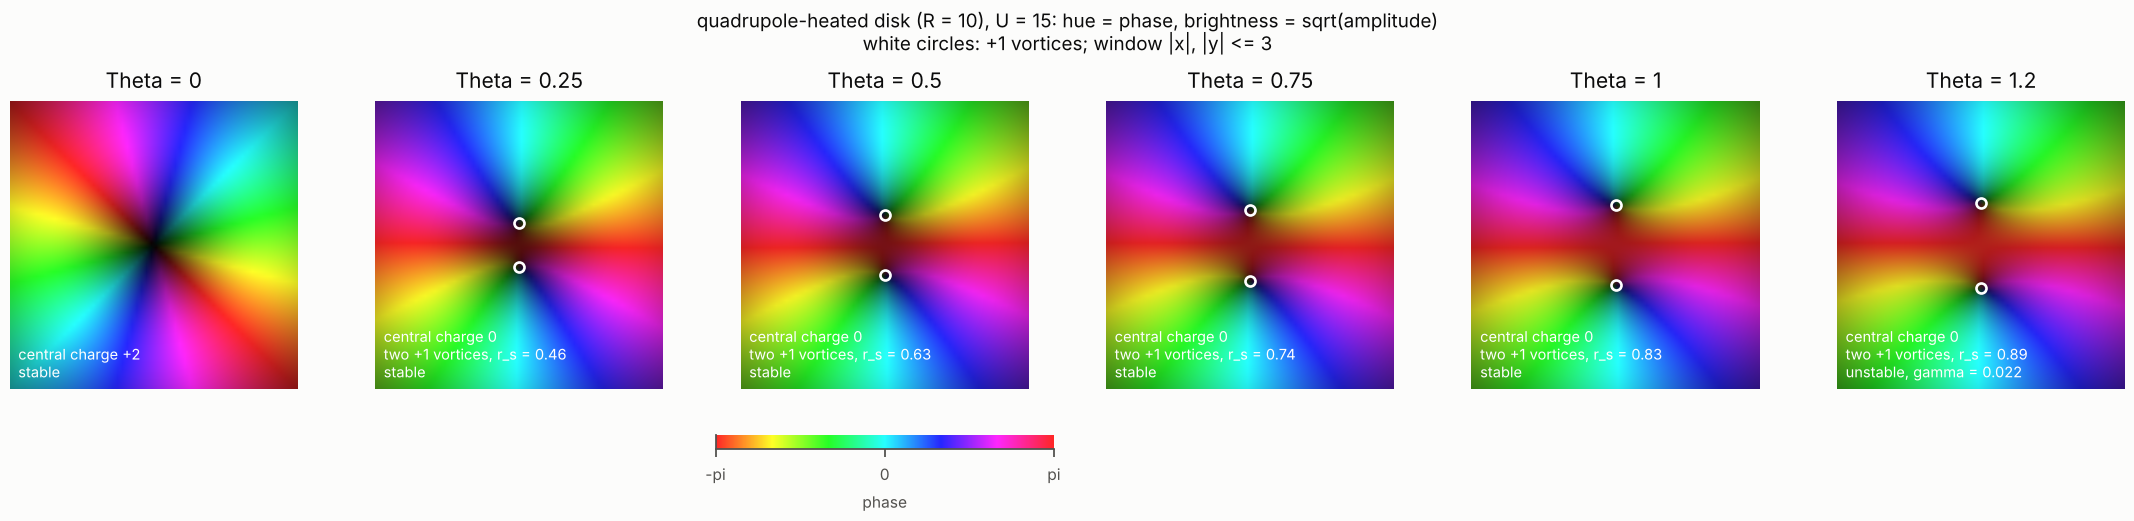
\includegraphics[width=0.98\textwidth,height=0.4\textheight,keepaspectratio]{twin_vortex_fields.png}
\par\medskip
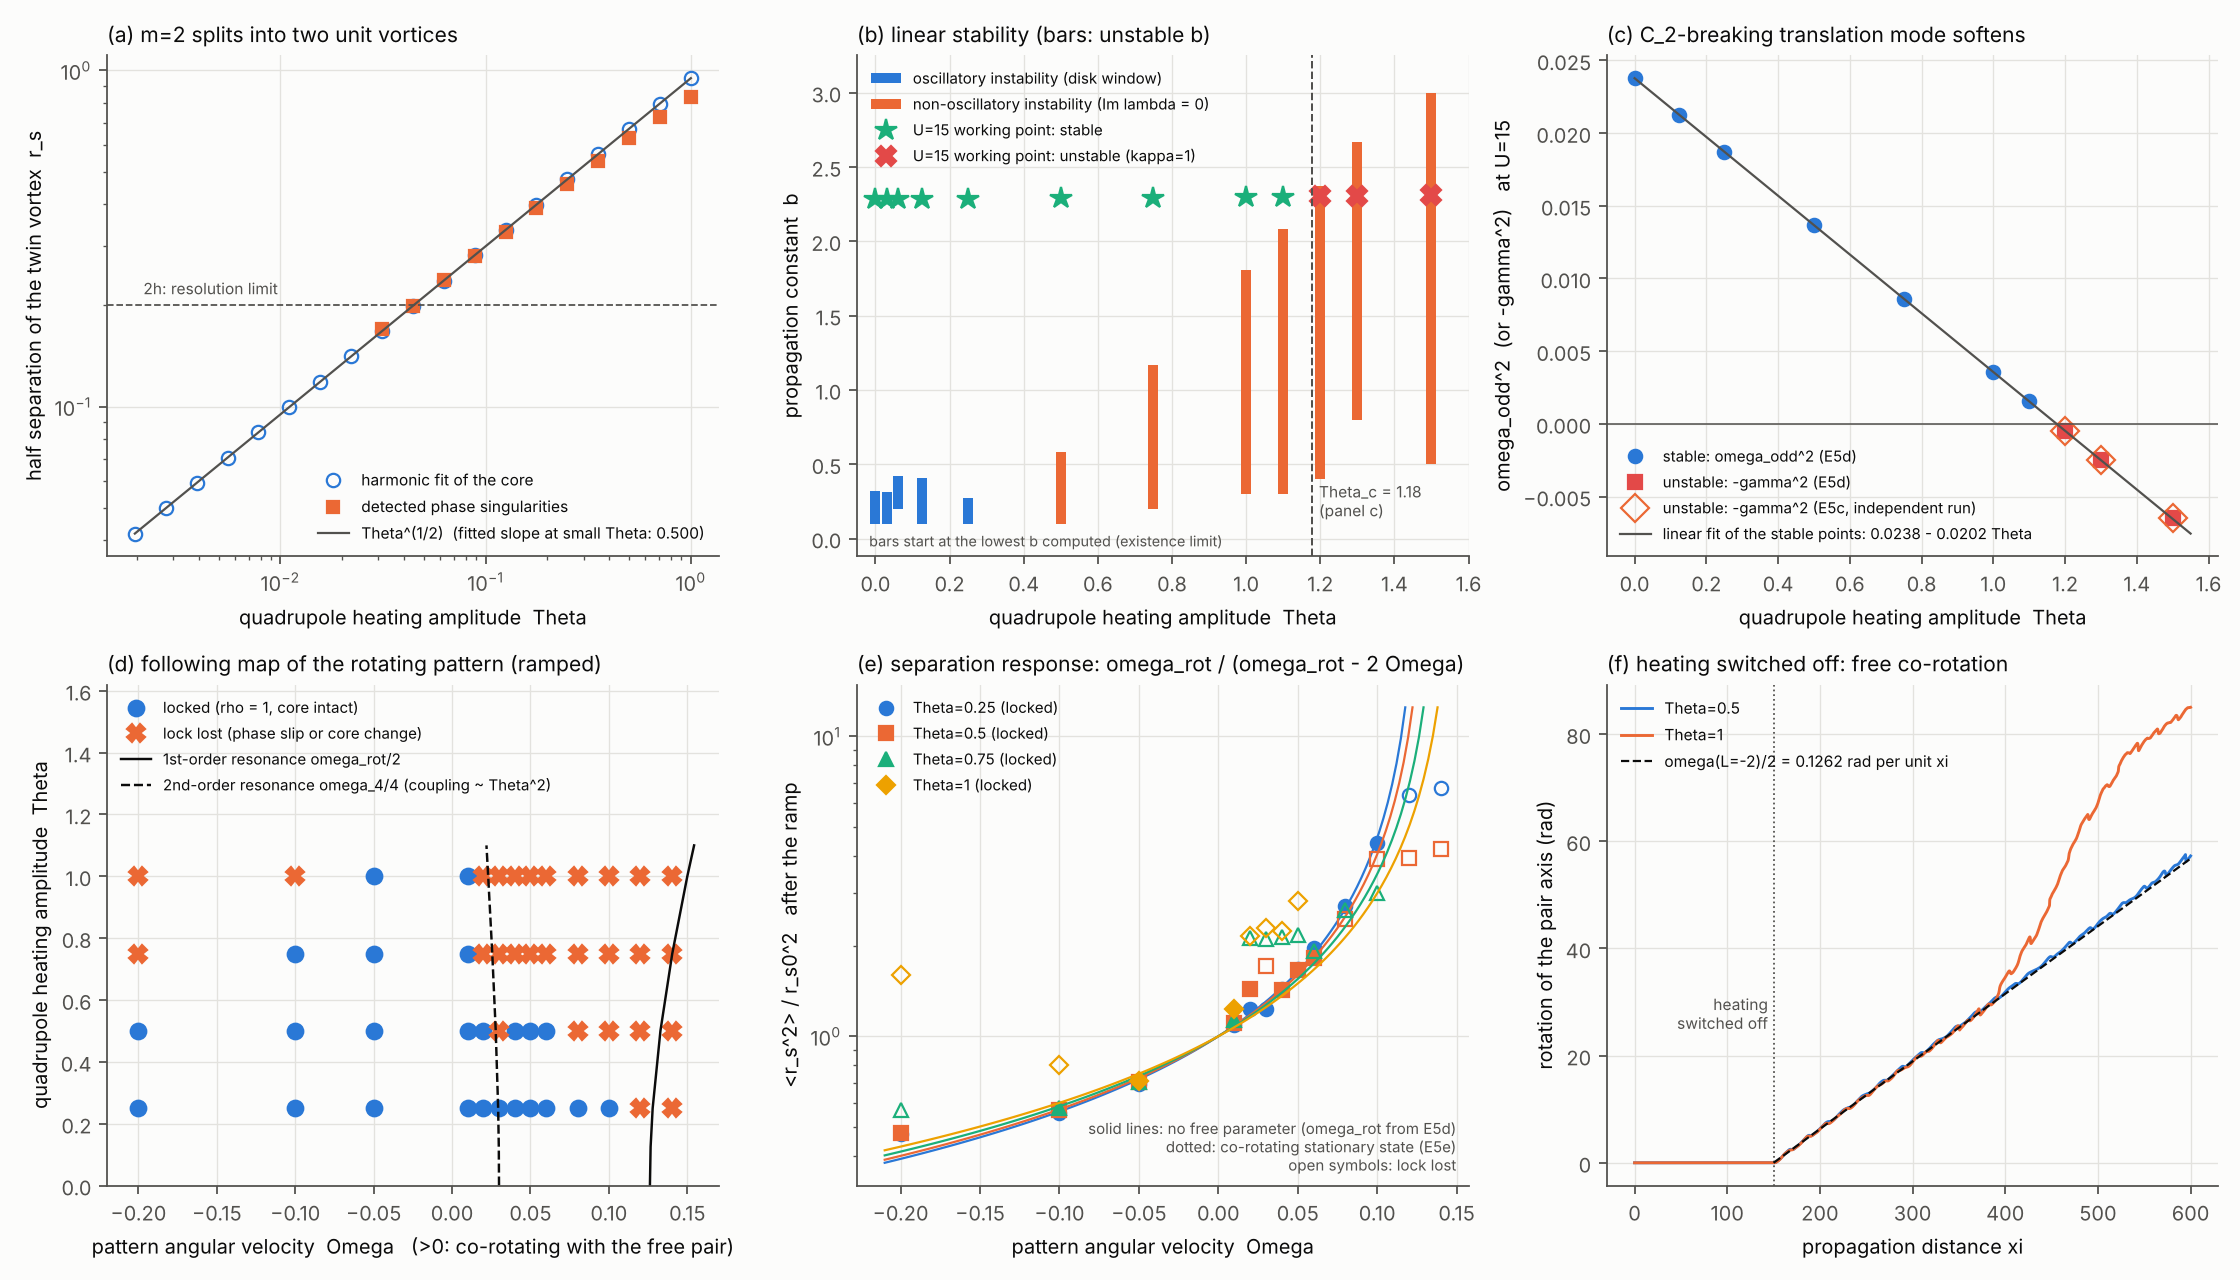
\includegraphics[width=0.98\textwidth,height=0.4\textheight,keepaspectratio]{twin_vortex.png}
\caption{\textbf{Thermally reconfigurable twin vortex} (disk \(R = 10\), \(U = 15\), quadrupolar heating \(\Theta \cos 2(\theta-\theta_0)\)). Top row: phase and amplitude for \(\Theta = 0\)--1.2, with central charge, half-separation and linear stability. (a) Half-separation \(r_s\) versus \(\Theta\), scaling as \(\Theta^{1/2}\). (b) Stability in the \((\Theta, b)\) plane, with the \(U = 15\) working points and \(\Theta_c\). (c) Squared frequency of the \(C_2\)-breaking translation mode, \(\omega_\mathrm{odd}^2\), versus \(\Theta\) (filled), and \(-\gamma^2\) from independent stability runs above \(\Theta_c\) (open). (d) Locking map: propagation with a ramped rotating pattern (circles: locked; crosses: lock lost) and rotating-frame stationary states (bands: stable in-phase branch and stable branch beyond a fold; thin lines: unstable, growth \(> 2\times10^{-3}\)), with the first- and second-order resonances \(\omega_\mathrm{rot}/2\) and \(\omega_{-4}/4\) and the line \(\Omega = -\omega_\mathrm{odd}(\Theta)\). (e) Separation response versus the parameter-free prediction \(\omega_\mathrm{rot}/(\omega_\mathrm{rot}-2\Omega)\) (solid lines); dotted: stable rotating-frame states. (f) Free co-rotation after the heating is switched off, compared with \(\omega_{-2}/2\).}
\label{fig6}
\end{figure}


\hypertarget{discussion}{%
\section{Discussion}\label{discussion}}

\textbf{Experimental scales.} For lead glass (\(n_0 \approx 1.8\), \(dn/dT \sim 10^{-5}\,\mathrm{K^{-1}}\)) at \(\lambda = 0.5\,\mu\)m and \(r_0 = 20\)--\(50\,\mu\)m:

\begin{itemize}
\tightlist
\item
  One unit of \(\xi\) is a diffraction length of about 0.5--6 cm, so the transmutation lengths \(\xi_t \approx 2\)--12 correspond to centimetre-scale samples.
\item
  \(\rho = 8\) or \(R = 10\) corresponds to sample radii of 0.2--0.5 mm.
\item
  One unit of \(N\) corresponds to \(\delta n \approx n_0/(k_0 r_0)^2 \approx 3\times10^{-5}\)--\(5\times10^{-6}\), so \(\Theta \approx 0.5\)--1 requires a boundary-temperature modulation of order 1 K. This is readily produced by segmented heaters or thermoelectric elements.
\end{itemize}

A rotating pattern corresponds to heaters whose orientation turns slowly along the sample. Treating the heat flow as transverse requires the pattern to vary along \(\xi\) much more slowly than transverse heat diffusion. The locking map is a property of the stationary states and does not depend on sample length. Over centimetre-scale samples, however, only instabilities with \(\gamma \gtrsim 0.1\) act, so the observable consequences in short samples are the tunable separation, Eq. (4), and the free co-rotation.

\textbf{Relation to other systems.} The intrinsic \(m = 2\) window and its widening by boundary symmetry are the optical counterpart of the splitting instability of doubly quantized vortices in condensates \citep{Skryabin2001, Mottonen2003split, Shin2004dqv, Lundh2006, Kapitula2013krein}. Here, however, the discrete symmetry and its strength are fixed by the sample boundary or set by heating. Anisotropy-induced splitting has been observed in photorefractive crystals \citep{Mamaev1997decay} and studied in anisotropic traps \citep{Mottonen2003split, Xiong2020ring}, but without a law for the separation; the \(\Theta^{1/2}\) law here follows from the forced response of the splitting mode. Pairs of like-signed vortices in rotating anisotropic traps align with the soft axis, and their separation decreases as the stirring frequency grows \citep{McEndoo2009, McEndoo2010}. Solitons set into rotation inside Bessel lattices, or carried by rotating lattices, remain trapped only below a critical angular velocity set by escape, depinning or force balance \citep{KVT2004rotary, Sakaguchi2007rotating, Cuevas2007rotating}. The twin vortex differs in two ways. It is a synchronous stationary state of a medium driven only at its boundary. And both of its locking limits are traced to identified internal modes: a resonance of the driven splitting mode and the zero crossing of the translation mode. It also differs from rotating dipoles and other spontaneously rotating nonlocal solitons \citep{LopezAguayo2006, Skupin2008}, whose rotation is intrinsic rather than imposed.

\textbf{Limitations.}

\begin{itemize}
\tightlist
\item
  Transmuted states with \(m \ge 3\) are unstable in all samples considered, so boundary design does not stabilize higher-order topology. It does make that topology observable over the transmutation length.
\item
  Structural conclusions for \(m \ge 4\) are limited by the grid's own \(C_4\) symmetry.
\item
  For \(n = 5, 6\) the shape anisotropy at \(\rho = 8\) is comparable to grid errors, so these rules are demonstrated by heating.
\end{itemize}

\hypertarget{conclusions}{%
\section{Conclusions}\label{conclusions}}

In a thermal nonlocal medium the sample boundary is a precise and tunable source of discrete rotational symmetry. An exact transfer law, \(\delta N \propto U (r/\rho)^n \cos n\theta\), and conformal-radius universality reduce any regular cross-section to a disk plus a known perturbation. A Newton-polygon selection rule then predicts the transmuted topology and its fractional scaling. The same symmetry, acting on the Bogoliubov spectrum through the selection rule \(\kappa = L \bmod n\), opens and widens instability windows whose edges follow from Hamilton--Hopf collisions. With boundary heating the design becomes reconfigurable: a quadrupolar pattern produces a twin vortex whose separation, stability limit, free rotation and response to a rotating pattern are all accounted for by one forced-splitting-mode picture. Its locking boundaries are a fold before a second-order resonance in one rotation direction and the zero crossing of the symmetry-breaking translation mode in the other.

\hypertarget{credit-authorship-contribution-statement}{%
\section*{CRediT authorship contribution statement}\label{credit-authorship-contribution-statement}}

{[}to be completed by the authors{]}

\hypertarget{declaration-of-competing-interest}{%
\section*{Declaration of competing interest}\label{declaration-of-competing-interest}}

The authors declare that they have no known competing financial interests or personal relationships that could have appeared to influence the work reported in this paper.

\hypertarget{data-availability}{%
\section*{Data availability}\label{data-availability}}

The code and the data underlying all figures will be made available at {[}repository to be added{]}.

\hypertarget{acknowledgments}{%
\section*{Acknowledgments}\label{acknowledgments}}

{[}to be added{]}

\appendix
\hypertarget{numerical-methods}{%
\section{Numerical methods}\label{numerical-methods}}

\begin{itemize}
\tightlist
\item
  \textbf{Grid and operators.} Cell-centred Cartesian grid, so that neither the origin nor the symmetry axes are grid lines. The Laplacian uses the isotropic nine-point stencil \(L_9 = \frac23 L_+ + \frac13 L_\times\), whose truncation error has no \(C_4\) component at \(O(h^2)\) \citep{Patra2006stencil}. The heat equation is discretized with the symmetric second-order Dirichlet treatment of Gibou et al. \citep{Gibou2002} on the true polygonal boundary. All operators are assembled edge by edge, so the matrices are exactly symmetric and the discrete Bogoliubov problem keeps its Hamiltonian structure.
\item
  \textbf{Stationary states.} Newton iteration on \((w_r, w_i, N)\) with sparse LU, at fixed \(b\) or fixed \(U\) (bordered system), with three globalization strategies and continuation with a secant predictor in \(b\), \(U\), \(\rho\) and \(\Theta\) \citep{Yang2009newton}. Residuals reach \(10^{-12}\) or the round-off floor.
\item
  \textbf{Stability.} Shift-invert Arnoldi on the full sample along \(\sigma = 0.02 + i\omega\). Each eigenvector is classified by its angular content (\(L\), \(\kappa\)) and Krein signature. The rotating-frame term \(-i\Omega\partial_\theta\) in Eq. (5) uses a fourth-order, exactly antisymmetric discretization.
\item
  \textbf{Propagation.} Crank--Nicolson for the linear part with Strang splitting for the nonlinear phase, and an exact heat solve at each step; power is conserved to \(10^{-13}\).
\item
  \textbf{Diagnostics.} Unit singularities are found by plaquette winding outside \(1.25h\) from the centre. The central charge is the winding on a circle of radius \(0.5h\). Sub-grid rings are characterized by a harmonic fit \(r_s = (|a_v|/|a_m|)^{1/(|m|-|v|)}\).
\end{itemize}

\hypertarget{controls-and-convergence}{%
\section{Controls and convergence}\label{controls-and-convergence}}

\begin{itemize}
\tightlist
\item
  \textbf{Grid convergence.} Key families were recomputed on a grid coarser by 1.5. Stability thresholds were followed on four grids (\(h = 0.15\), 0.1, 0.075, 0.05) and extrapolated in \(h^2\).
\item
  \textbf{Rotation test.} Rotating a polygon by \(15^\circ\) relative to the grid leaves thresholds and growth rates unchanged to three digits.
\item
  \textbf{Resolution floor.} Disk controls for \(m \ge 4\) show the grid-induced \(C_4\) splitting (\(r \approx 0.28\) for \(m = 4\) at \(h = 0.1\)), which does not decrease monotonically with \(h\). All conclusions for \(m \ge 4\) are compared against these controls.
\item
  \textbf{Independent radial solver.} For the disk, rotational symmetry reduces the stationary problem and each Bogoliubov channel \(L\) to radial equations. We solve them with a second-order finite-volume scheme on a cell-centred radial grid and eliminate the nonlocal response exactly through the radial Green matrix; the method shares no code and no grid with the Cartesian solver. It reproduces the phase zero mode, the power curves \(U(b)\) of the \(m = 1\)--3 families of the Cartesian solver to within 0.2\%, and the \(m = 3\) growth rates (0.068 at \(b = 0.2\) and 0.232 at \(b = 7\), against 0.067 and 0.229 on the Cartesian grid with \(h = 0.1\)). It gives the window edges \(bR^2 = 8.25\) (\(m = 1\), \(L = -1\)) and \(32.56\) (\(m = 2\), \(L = -2\)), converged to \(10^{-4}\) in \(b\) between 600 and 1200 radial cells, and a weaker, subdominant \(L = -1\) instability of \(m = 2\) for \(bR^2 < 13.7\) (Fig. S1).
\item
  \textbf{Seeded propagation.} Displacing the input beam by \(10^{-3}\) seeds the \(C_2\)-breaking translation mode. The growth rate is fitted to the last two decades of exponential growth before nonlinear saturation and before any change of the core, because the seed also excites non-growing \(C_2\)-breaking modes that dominate the early evolution (Fig. S2).
\item
  \textbf{Reproduction of earlier results.} The twin vortex in rectangles and the instability of \(m \ge 3\) \citep{Ye2010twin}, and surface dipoles and vortices \citep{Ye2008surface}, are reproduced.
\item
  \textbf{Twin-vortex results.} The locking classification and the free co-rotation rate (0.2191 vs 0.21904 at \(\Theta = 1\)) agree between \(h = 0.1\) and \(h = 0.075\).
\end{itemize}

\section{Supplementary figures}
\renewcommand{\thefigure}{S\arabic{figure}}\setcounter{figure}{0}
\begin{figure}[tbp]
\centering
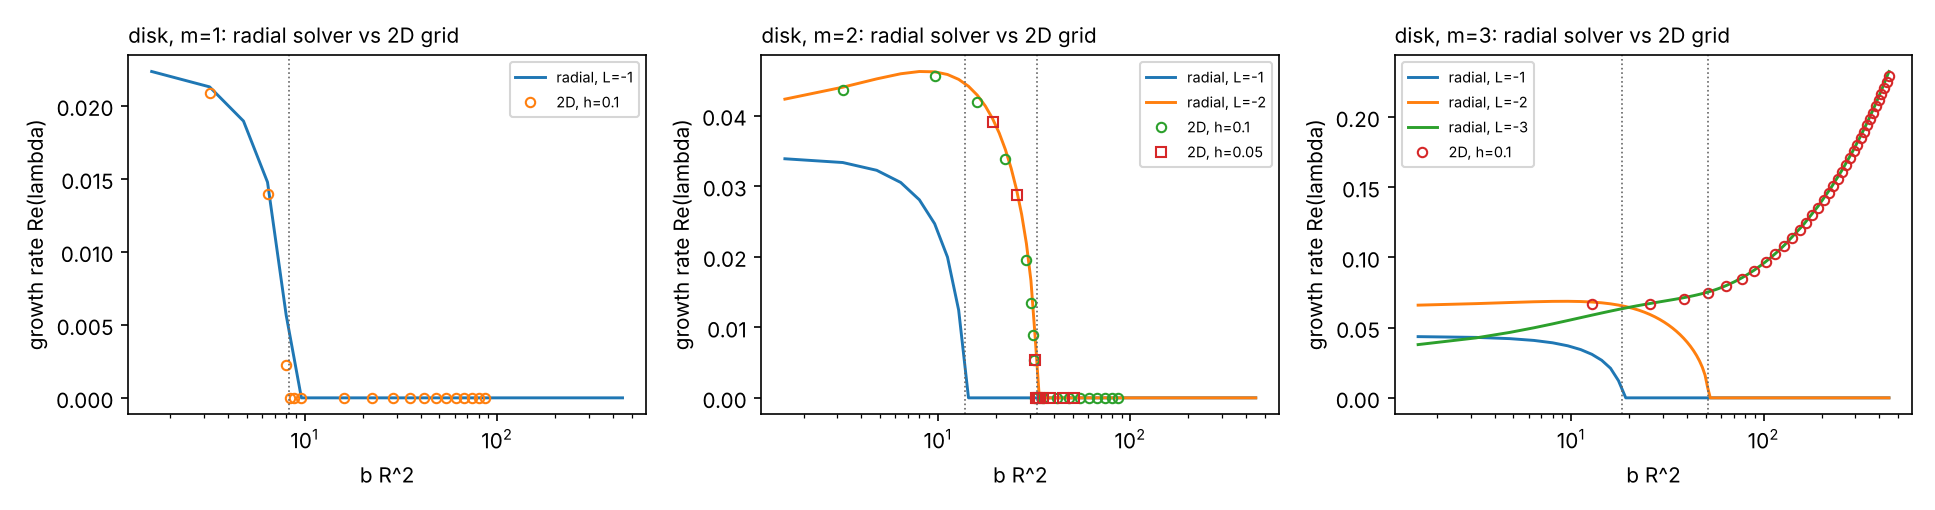
\includegraphics[width=0.98\textwidth,height=0.72\textheight,keepaspectratio]{e3c_radial_vs_2d.png}
\caption{\textbf{Independent radial check of the disk windows.} Growth rates of the \(m = 1\), 2, 3 vortices in a disk of radius \(R = 8\) versus \(bR^2\), from the radial solver (lines, one per channel \(L\)) and from the Cartesian solver at \(h = 0.1\) and \(0.05\) (symbols). Dotted lines mark the converged window edges.}
\label{figS1}
\end{figure}
\begin{figure}[tbp]
\centering
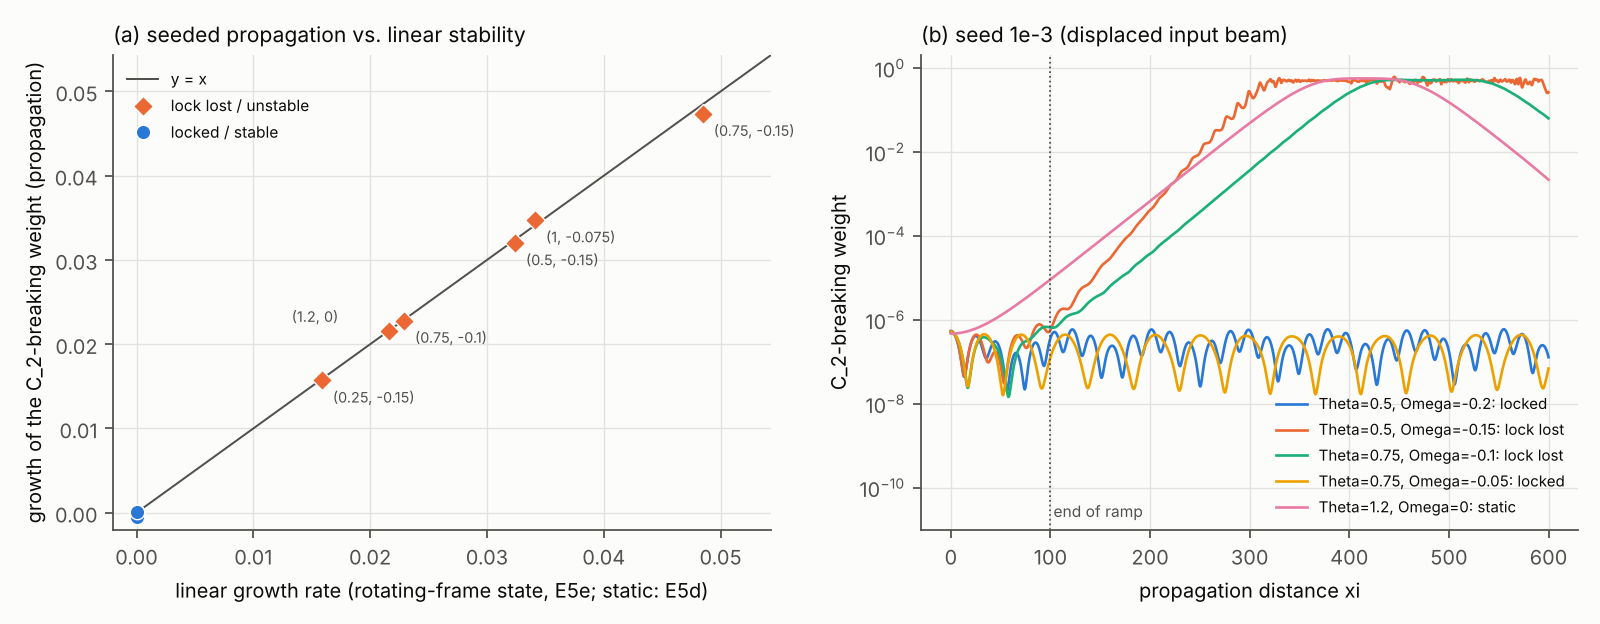
\includegraphics[width=0.98\textwidth,height=0.72\textheight,keepaspectratio]{twin_vortex_seed.png}
\caption{\textbf{Seeded propagation.} (a) Growth rate of the \(C_2\)-breaking weight in propagation with the input beam displaced by \(10^{-3}\), against the linear growth rate of the rotating-frame state (static points: linear stability of the heated state). Diamonds: lock lost or unstable; circles: locked or stable. (b) \(C_2\)-breaking weight versus \(\xi\) for representative points; the pattern is accelerated over \(\xi \le 100\).}
\label{figS2}
\end{figure}


\bibliographystyle{elsarticle-num}
\bibliography{refs}
\end{document}
